% TikZ Diagram: Unified closed-form engine across LTSF & scientific chaos
% Style: Minimal publication palette (Grayscale structural + Single Accent for proposed module)
% Rules: Rectangles = Operations/Modules, Rounded = Data/Tensors. Left-to-right flow. Zero line crossing.

\documentclass[tikz,border=10pt]{standalone}
\usetikzlibrary{shapes.geometric, positioning, arrows.meta, chains, backgrounds}

\definecolor{neutralbg}{HTML}{F8FAFC}
\definecolor{neutralstroke}{HTML}{64748B}
\definecolor{neutraltext}{HTML}{0F172A}

\definecolor{accentbg}{HTML}{FEF3C7}
\definecolor{accentstroke}{HTML}{D97706}
\definecolor{accenttext}{HTML}{92400E}

\begin{document}
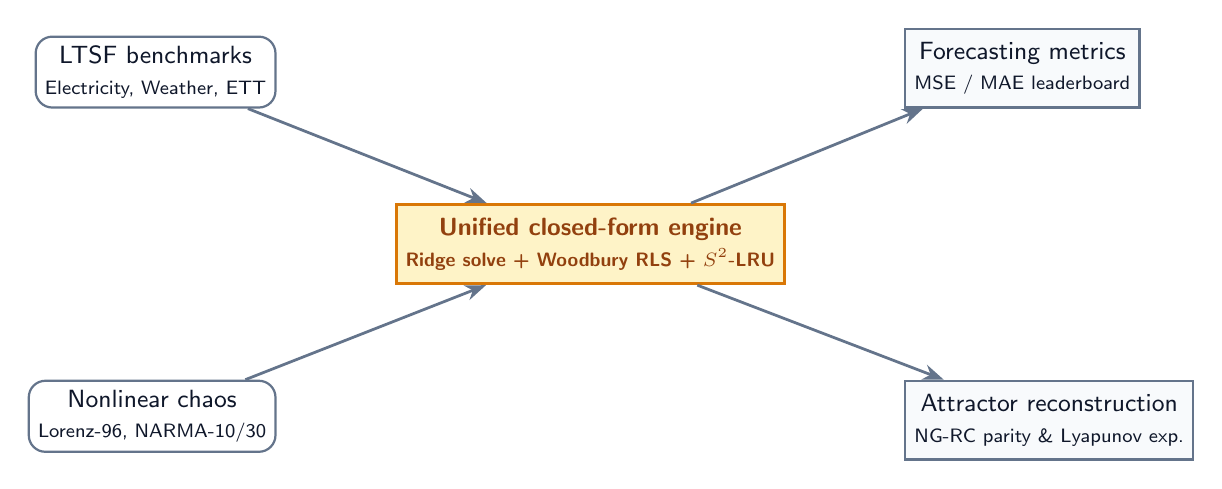
\begin{tikzpicture}[
    font=\sffamily\small,
    node distance=1.0cm and 1.2cm,
    operation/.style={rectangle, draw=neutralstroke, fill=neutralbg, text=neutraltext, minimum height=1.0cm, minimum width=2.2cm, align=center, line width=0.8pt},
    proposed_op/.style={rectangle, draw=accentstroke, fill=accentbg, text=accenttext, minimum height=1.0cm, minimum width=2.4cm, align=center, line width=1.2pt, font=\sffamily\bfseries\small},
    tensor/.style={rounded corners=6pt, draw=neutralstroke, fill=white, text=neutraltext, minimum height=0.9cm, minimum width=2.0cm, align=center, line width=0.8pt},
    proposed_tensor/.style={rounded corners=6pt, draw=accentstroke, fill=accentbg!50, text=accenttext, minimum height=0.9cm, minimum width=2.2cm, align=center, line width=1.0pt},
    arrow/.style={-{Stealth[scale=1.0]}, line width=1.0pt, draw=neutralstroke},
    aux_arrow/.style={-{Stealth[scale=1.0]}, line width=1.0pt, draw=accentstroke, dashed}
]

    % Proposed unified solver core
    \node[proposed_op] (core) {Unified closed-form engine\\{\scriptsize Ridge solve + Woodbury RLS + $S^2$-LRU}};

    % Domain 1: LTSF
    \node[tensor, above left=1.2cm and 1.5cm of core] (ltsf_data) {LTSF benchmarks\\{\scriptsize Electricity, Weather, ETT}};
    \node[operation, above right=1.2cm and 1.5cm of core] (ltsf_metric) {Forecasting metrics\\{\scriptsize MSE / MAE leaderboard}};

    % Domain 2: Chaos
    \node[tensor, below left=1.2cm and 1.5cm of core] (chaos_data) {Nonlinear chaos\\{\scriptsize Lorenz-96, NARMA-10/30}};
    \node[operation, below right=1.2cm and 1.5cm of core] (chaos_metric) {Attractor reconstruction\\{\scriptsize NG-RC parity \& Lyapunov exp.}};

    % Flow arrows
    \draw[arrow] (ltsf_data) -- (core);
    \draw[arrow] (core) -- (ltsf_metric);
    \draw[arrow] (chaos_data) -- (core);
    \draw[arrow] (core) -- (chaos_metric);

\end{tikzpicture}
\end{document}
